\section{error control instead of defect control}
Another idea is to consider error control instead of defect control for the continuous approximate solution. We would thus need a way to create two interpolants, one of a higher order and one of a lower order and sample the difference between these two interpolants to estimate the error of the continuous solution approximation. 
=== A step-size selection algorithm based on that error estimate could provide an effective error controlled solution.

An issue with defect control is the V-shape of the defect. 
We know that this is entirely because of the $\frac{1}{h}$ in the derivative definition of the Hermite-Birkhoff interpolants as the interpolant itself does not suffer from round-off error but its derivative does.

\subsection{error is not v-shaped}
For all the schemes, the defect is V-shaped but the error itself is not. 
This is because the Hermite-Birkhoff interpolant does not contain a term in $\frac{1}{h}$ whereas its derivative does contain such a term. 
Figure $\ref{fig:defect_is_v_shape}$ and $\ref{fig:error_is_not_v_shape}$ shows this phenomenon for HB6 but the same can be see for HB4 and HB8. 

\begin{figure}[H]
\centering
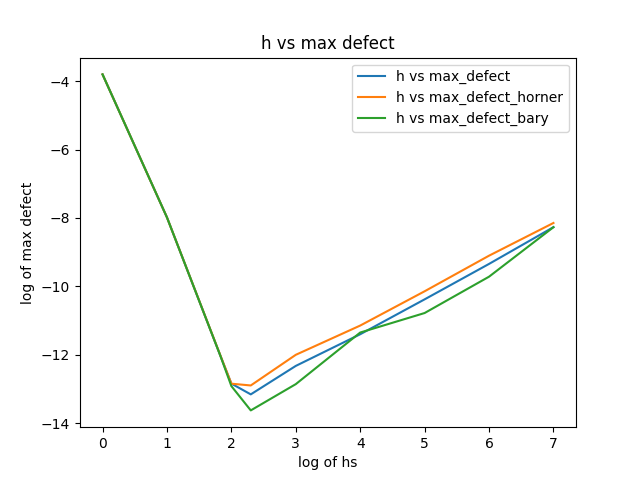
\includegraphics[width=0.7\linewidth]{./figures/further_work_defect_is_v_shape_hb6}
\caption{Defect has V-shape.}
\label{fig:defect_is_v_shape}
\end{figure}

\begin{figure}[H]
\centering
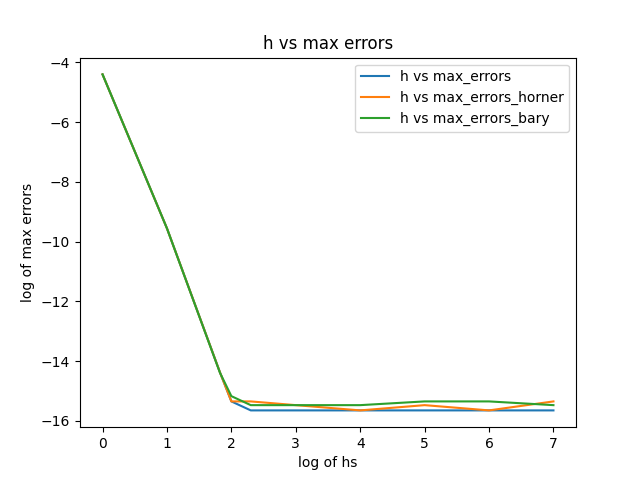
\includegraphics[width=0.7\linewidth]{./figures/further_work_error_is_not_v_shape_hb6}
\caption{Error does not have V-shape.}
\label{fig:error_is_not_v_shape}
\end{figure}

\subsection{sampling error}
we sample
\begin{equation}
| h(x) - l(x) |
\end{equation}
at two x values within $x_i$ and $x_{i+1}$ and take the max to get the error estimate within the step.

\subsubsection{rk4 with hb4 vs hb6 with sampling}
Because we do not differentiate and that hb4 has order 4, we can use with rk4 with HB4 for error control. Thus HB4 and HB6 should not suffer from much interpolation error and we can use rk4 with the hb4 and hb6 using the error scheme

\paragraph{Problem 1} Figures $\ref{fig:rk4_with_hb4_hb6_sampling_p1_global_error}$ and $\ref{fig:rk4_with_hb4_hb6_sampling_p1_scaled_errors}$ shows the global error and the shape of the error on each step of using rk4 with hb4 vs hb6 with sampling on Problem 1 at an absolute tolerance of $10^{-6}$. From Figure $\ref{fig:rk4_with_hb4_hb6_sampling_p1_scaled_errors}$, we can see that there is no consistent location where we can sample the error to get the maximum error.

\begin{figure}[H]
\centering
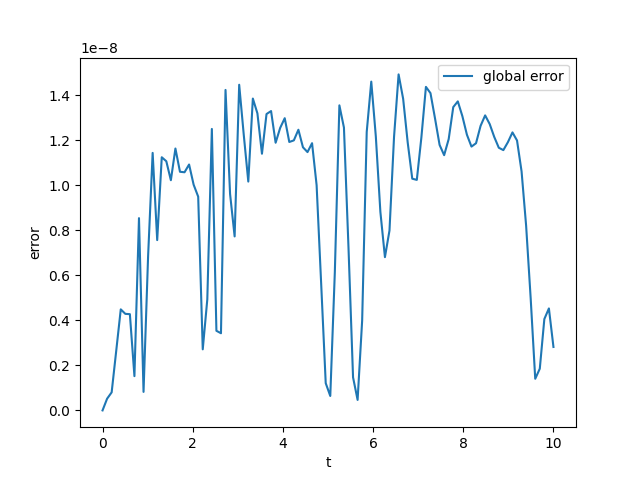
\includegraphics[width=0.7\linewidth]{./figures/rk4_with_hb4_hb6_sampling_p1_global_error}
\caption{Global Error for RK4 with HB4 vs HB6 with error sampling on problem 1 at an absolute tolerance of $10^{-6}$.}
\label{fig:rk4_with_hb4_hb6_sampling_p1_global_error}
\end{figure}

\begin{figure}[H]
\centering
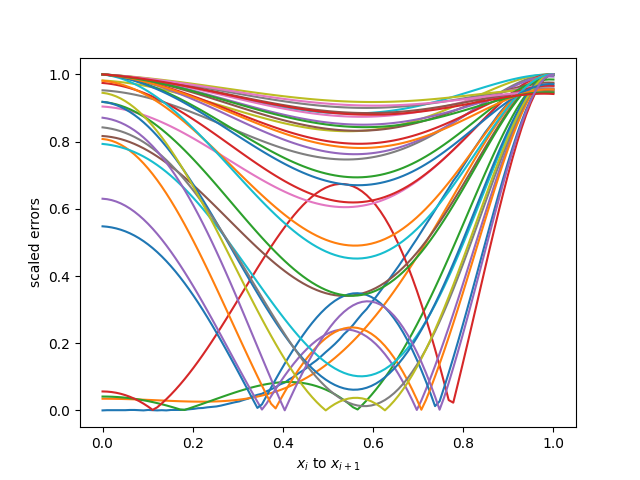
\includegraphics[width=0.7\linewidth]{./figures/rk4_with_hb4_hb6_sampling_p1_scaled_errors}
\caption{Scaled errors over all steps for RK4 with HB4 vs HB6 with error sampling on problem 1 at an absolute tolerance of $10^{-6}$ mapped onto $[0, 1]$.}
\label{fig:rk4_with_hb4_hb6_sampling_p1_scaled_errors}
\end{figure}

\paragraph{Problem 2} Figures $\ref{fig:rk4_with_hb4_hb6_sampling_p2_global_error}$ and $\ref{fig:rk4_with_hb4_hb6_sampling_p2_scaled_errors}$ shows the global error and the shape of the error on each step of using rk4 with hb4 vs hb6 with sampling on Problem 2 at an absolute tolerance of $10^{-6}$. From Figure $\ref{fig:rk4_with_hb4_hb6_sampling_p2_scaled_errors}$, we can see that there is no consistent location where we can sample the error to get the maximum error.

\begin{figure}[H]
\centering
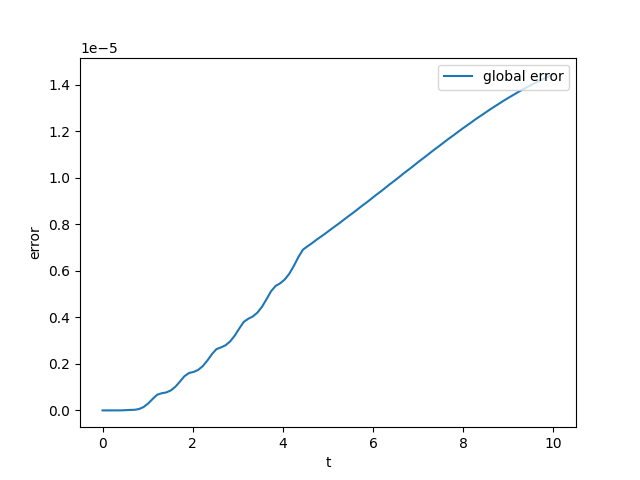
\includegraphics[width=0.7\linewidth]{./figures/rk4_with_hb4_hb6_sampling_p2_global_error}
\caption{Global Error for RK4 with HB4 vs HB6 with error sampling on problem 2 at an absolute tolerance of $10^{-6}$.}
\label{fig:rk4_with_hb4_hb6_sampling_p2_global_error}
\end{figure}

\begin{figure}[H]
\centering
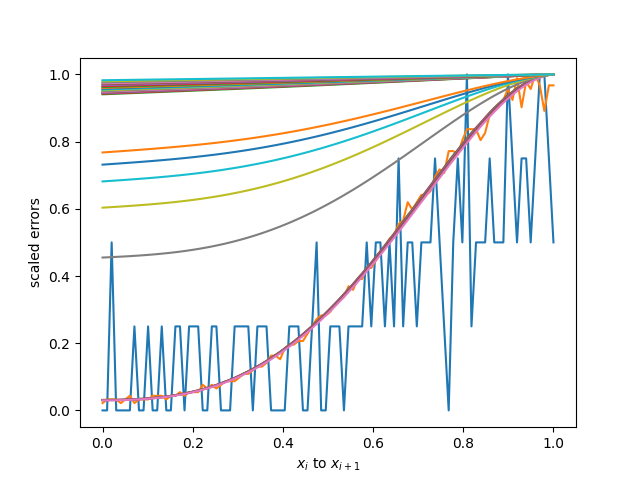
\includegraphics[width=0.7\linewidth]{./figures/rk4_with_hb4_hb6_sampling_p2_scaled_errors}
\caption{Scaled errors over all steps for RK4 with HB4 vs HB6 with error sampling on problem 2 at an absolute tolerance of $10^{-6}$ mapped onto $[0, 1]$.}
\label{fig:rk4_with_hb4_hb6_sampling_p2_scaled_errors}
\end{figure}

\paragraph{Problem 3} Figures $\ref{fig:rk4_with_hb4_hb6_sampling_p3_global_error}$ and $\ref{fig:rk4_with_hb4_hb6_sampling_p3_scaled_errors}$ shows the global error and the shape of the error on each step of using rk4 with hb4 vs hb6 with sampling on Problem 3 at an absolute tolerance of $10^{-6}$. From Figure $\ref{fig:rk4_with_hb4_hb6_sampling_p3_scaled_errors}$, we can see that there is no consistent location where we can sample the error to get the maximum error.

\begin{figure}[H]
\centering
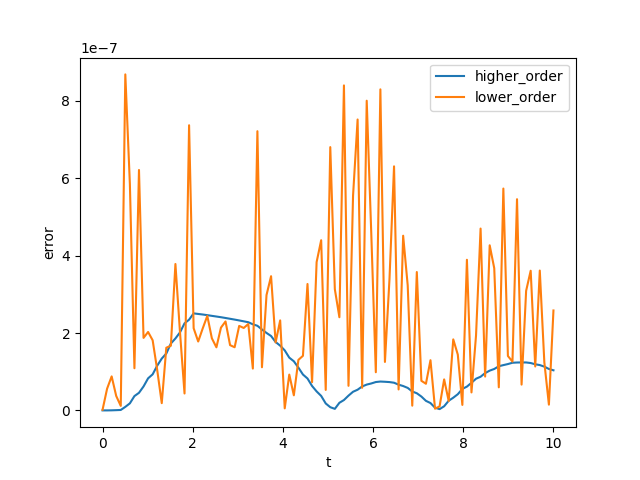
\includegraphics[width=0.7\linewidth]{./figures/rk4_with_hb4_hb6_sampling_p3_global_error}
\caption{Global Error for RK4 with HB4 vs HB6 with error sampling on problem 3 at an absolute tolerance of $10^{-6}$.}
\label{fig:rk4_with_hb4_hb6_sampling_p3_global_error}
\end{figure}

\begin{figure}[H]
\centering
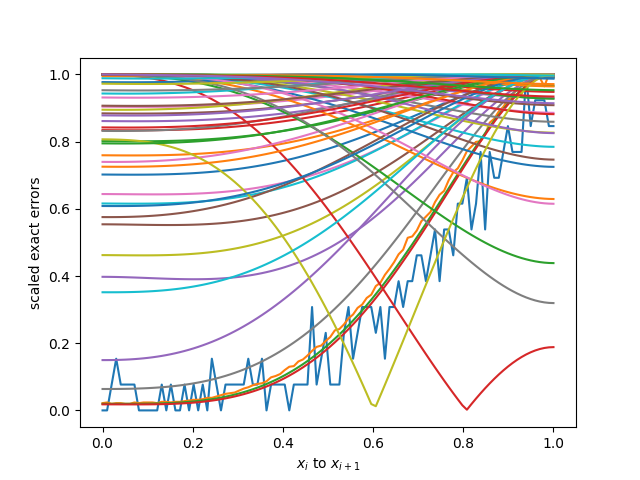
\includegraphics[width=0.7\linewidth]{./figures/rk4_with_hb4_hb6_sampling_p3_scaled_errors}
\caption{Scaled errors over all steps for RK4 with HB4 vs HB6 with error sampling on problem 3 at an absolute tolerance of $10^{-6}$ mapped onto $[0, 1]$.}
\label{fig:rk4_with_hb4_hb6_sampling_p3_scaled_errors}
\end{figure}

\begin{table}[h]
\caption {Number of steps taken by RK4 using error control with HB4 vs HB6 by sampling the error.} \label{tab:rk4_with_hb4_hb6_sampling_nsteps}
\begin{center}
\begin{tabular}{ c c c } 
Problem & successful steps & total steps \\ 
1       & 35                         & 37 \\ 
2       & 30                         & 34 \\
3       & 75                         & 97 \\
\end{tabular}
\end{center}
\end{table}


\subsubsection{rk4 with hb6 vs hb8 with sampling}
rk4 can also be use with hb6  and hb8 and not suffer from much interpolation error.

\paragraph{Problem 1} Figures $\ref{fig:rk4_with_hb6_hb8_sampling_p1_global_error}$ and $\ref{fig:rk4_with_hb6_hb8_sampling_p1_scaled_errors}$ shows the global error and the shape of the error on each step of using rk4 with hb6 vs hb8 with sampling on Problem 1 at an absolute tolerance of $10^{-6}$. From Figure $\ref{fig:rk4_with_hb6_hb8_sampling_p1_scaled_errors}$, we can see that there is no consistent location where we can sample the error to get the maximum error.

\begin{figure}[H]
\centering
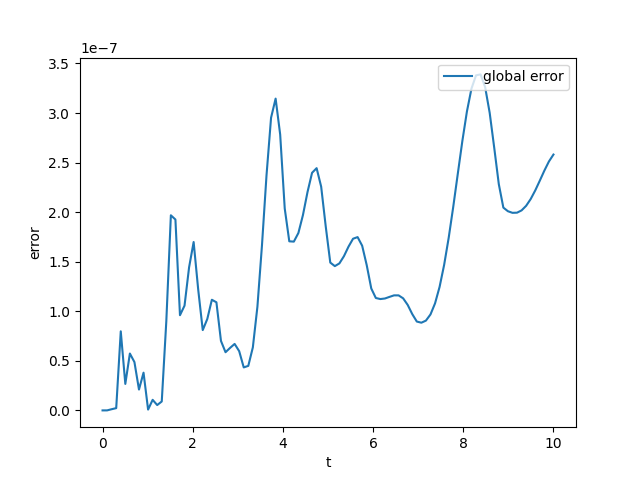
\includegraphics[width=0.7\linewidth]{./figures/rk4_with_hb6_hb8_sampling_p1_global_error}
\caption{Global Error for RK4 with HB6 vs HB8 with error sampling on problem 1 at an absolute tolerance of $10^{-6}$.}
\label{fig:rk4_with_hb6_hb8_sampling_p1_global_error}
\end{figure}

\begin{figure}[H]
\centering
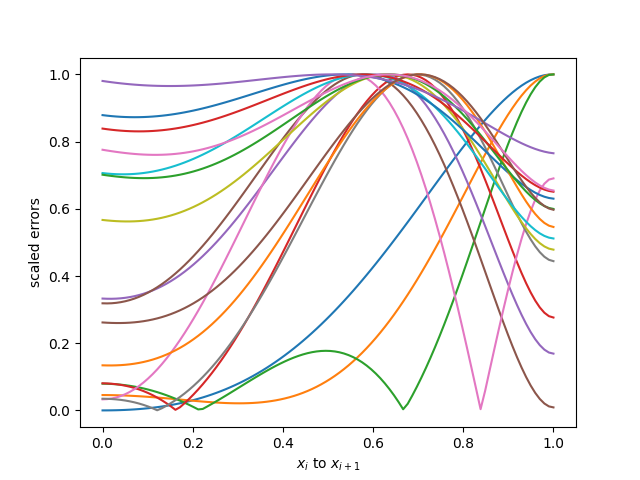
\includegraphics[width=0.7\linewidth]{./figures/rk4_with_hb6_hb8_sampling_p1_scaled_errors}
\caption{Scaled errors over all steps for RK4 with HB6 vs HB8 with error sampling on problem 1 at an absolute tolerance of $10^{-6}$ mapped onto $[0, 1]$.}
\label{fig:rk4_with_hb6_hb8_sampling_p1_scaled_errors}
\end{figure}

\paragraph{Problem 2} Figures $\ref{fig:rk4_with_hb6_hb8_sampling_p2_global_error}$ and $\ref{fig:rk4_with_hb6_hb8_sampling_p2_scaled_errors}$ shows the global error and the shape of the error on each step of using rk4 with hb6 vs hb8 with sampling on Problem 2 at an absolute tolerance of $10^{-6}$. From Figure $\ref{fig:rk4_with_hb6_hb8_sampling_p2_scaled_errors}$, we can see that there is no consistent location where we can sample the error to get the maximum error.

\begin{figure}[H]
\centering
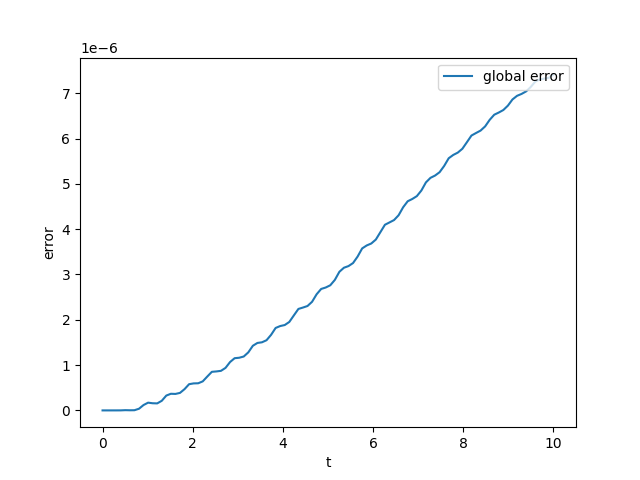
\includegraphics[width=0.7\linewidth]{./figures/rk4_with_hb6_hb8_sampling_p2_global_error}
\caption{Global Error for RK4 with HB6 vs HB8 with error sampling on problem 2 at an absolute tolerance of $10^{-6}$.}
\label{fig:rk4_with_hb6_hb8_sampling_p2_global_error}
\end{figure}

\begin{figure}[H]
\centering
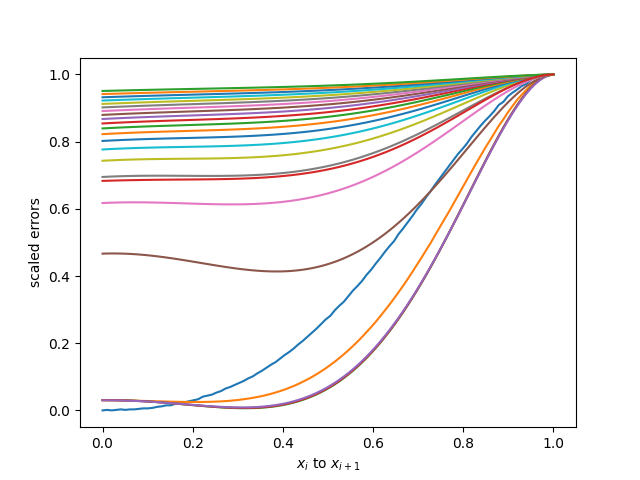
\includegraphics[width=0.7\linewidth]{./figures/rk4_with_hb6_hb8_sampling_p2_scaled_errors}
\caption{Scaled errors over all steps for RK4 with HB6 vs HB8 with error sampling on problem 2 at an absolute tolerance of $10^{-6}$ mapped onto $[0, 1]$.}
\label{fig:rk4_with_hb6_hb8_sampling_p2_scaled_errors}
\end{figure}

\paragraph{Problem 3} Figures $\ref{fig:rk4_with_hb6_hb8_sampling_p3_global_error}$ and $\ref{fig:rk4_with_hb6_hb8_sampling_p3_scaled_errors}$ shows the global error and the shape of the error on each step of using rk4 with hb6 vs hb8 with sampling on Problem 3 at an absolute tolerance of $10^{-6}$. From Figure $\ref{fig:rk4_with_hb6_hb8_sampling_p3_scaled_errors}$, we can see that there is no consistent location where we can sample the error to get the maximum error.

\begin{figure}[H]
\centering
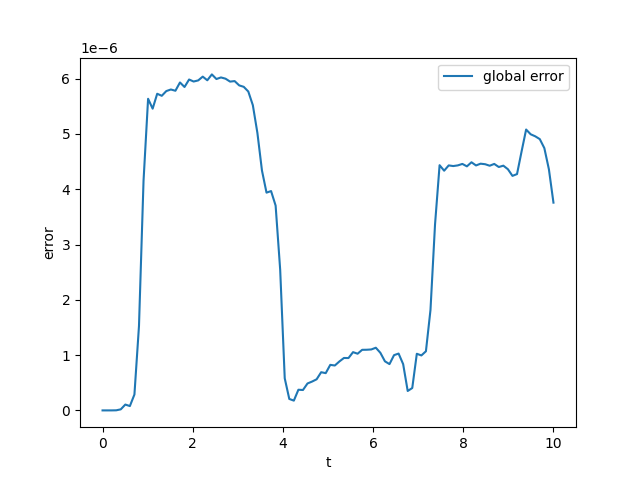
\includegraphics[width=0.7\linewidth]{./figures/rk4_with_hb6_hb8_sampling_p3_global_error}
\caption{Global Error for RK4 with HB6 vs HB8 with error sampling on problem 3 at an absolute tolerance of $10^{-6}$.}
\label{fig:rk4_with_hb6_hb8_sampling_p3_global_error}
\end{figure}

\begin{figure}[H]
\centering
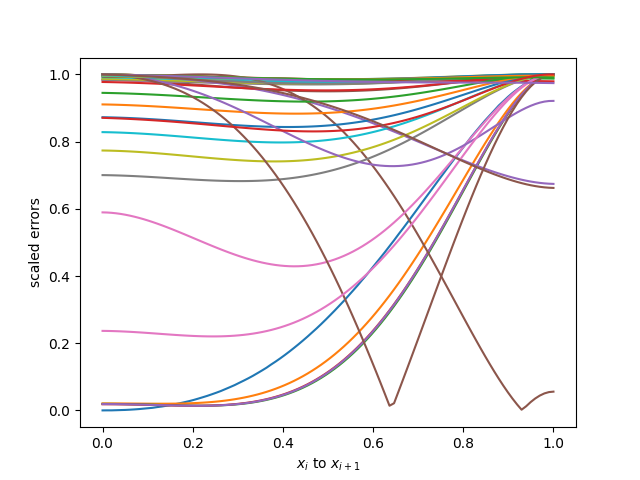
\includegraphics[width=0.7\linewidth]{./figures/rk4_with_hb6_hb8_sampling_p3_scaled_errors}
\caption{Scaled errors over all steps for RK4 with HB6 vs HB8 with error sampling on problem 3 at an absolute tolerance of $10^{-6}$ mapped onto $[0, 1]$.}
\label{fig:rk4_with_hb6_hb8_sampling_p3_scaled_errors}
\end{figure}

\begin{table}[h]
\caption {Number of steps taken by RK4 using error control with HB6 vs HB8 by sampling the error.} \label{tab:rk4_with_hb6_hb8_sampling_nsteps}
\begin{center}
\begin{tabular}{ c c c } 
Problem & successful steps & total steps \\ 
1       & 17                         & 17 \\ 
2       & 24                         & 42 \\
3       & 36                         & 57 \\
\end{tabular}
\end{center}
\end{table}

\subsubsection{rk6 with hb6 vs hb8 with sampling}
Because we do not differentiate and that hb6 has order 6, we can use with rk6 with HB6 for error control. Thus HB6 and HB8 should not suffer from much interpolation error and we can use rk6 with the hb4 and hb6 using the error scheme

\paragraph{Problem 1} Figures $\ref{fig:rk6_with_hb6_hb8_sampling_p1_global_error}$ and $\ref{fig:rk6_with_hb6_hb8_sampling_p1_scaled_errors}$ shows the global error and the shape of the error on each step of using rk6 with hb6 vs hb8 with sampling on Problem 1 at an absolute tolerance of $10^{-6}$. From Figure $\ref{fig:rk6_with_hb6_hb8_sampling_p1_scaled_errors}$, we can see that there is no consistent location where we can sample the error to get the maximum error.

\begin{figure}[H]
\centering
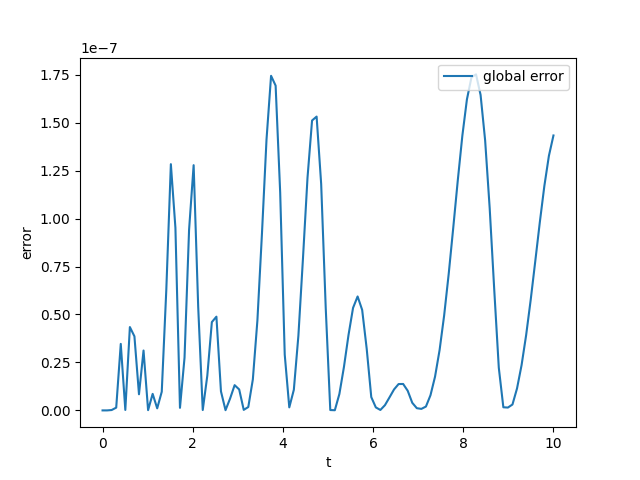
\includegraphics[width=0.7\linewidth]{./figures/rk6_with_hb6_hb8_sampling_p1_global_error}
\caption{Global Error for RK6 with HB6 vs HB8 with error sampling on problem 1 at an absolute tolerance of $10^{-6}$.}
\label{fig:rk6_with_hb6_hb8_sampling_p1_global_error}
\end{figure}

\begin{figure}[H]
\centering
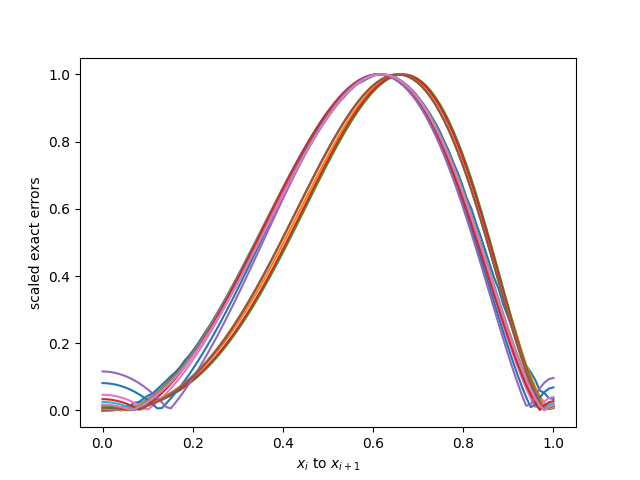
\includegraphics[width=0.7\linewidth]{./figures/rk6_with_hb6_hb8_sampling_p1_scaled_errors}
\caption{Scaled errors over all steps for RK6 with HB6 vs HB8 with error sampling on problem 1 at an absolute tolerance of $10^{-6}$ mapped onto $[0, 1]$.}
\label{fig:rk6_with_hb6_hb8_sampling_p1_scaled_errors}
\end{figure}

\paragraph{Problem 2} Figures $\ref{fig:rk6_with_hb6_hb8_sampling_p2_global_error}$ and $\ref{fig:rk6_with_hb6_hb8_sampling_p2_scaled_errors}$ shows the global error and the shape of the error on each step of using rk6 with hb6 vs hb8 with sampling on Problem 2 at an absolute tolerance of $10^{-6}$. From Figure $\ref{fig:rk6_with_hb6_hb8_sampling_p2_scaled_errors}$, we can see that there is no consistent location where we can sample the error to get the maximum error.

\begin{figure}[H]
\centering
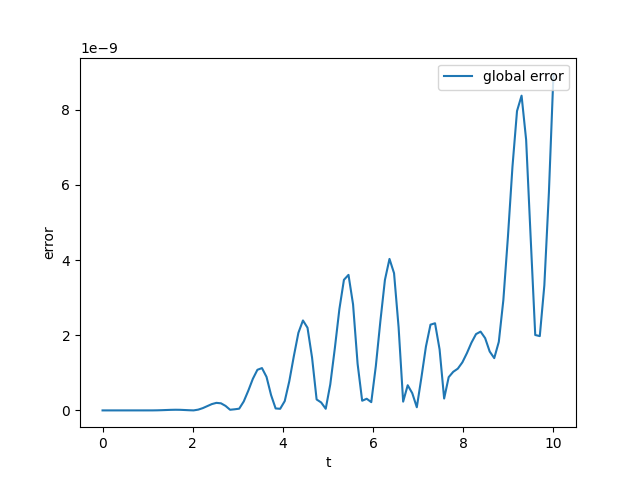
\includegraphics[width=0.7\linewidth]{./figures/rk6_with_hb6_hb8_sampling_p2_global_error}
\caption{Global Error for RK6 with HB6 vs HB8 with error sampling on problem 2 at an absolute tolerance of $10^{-6}$.}
\label{fig:rk6_with_hb6_hb8_sampling_p2_global_error}
\end{figure}

\begin{figure}[H]
\centering
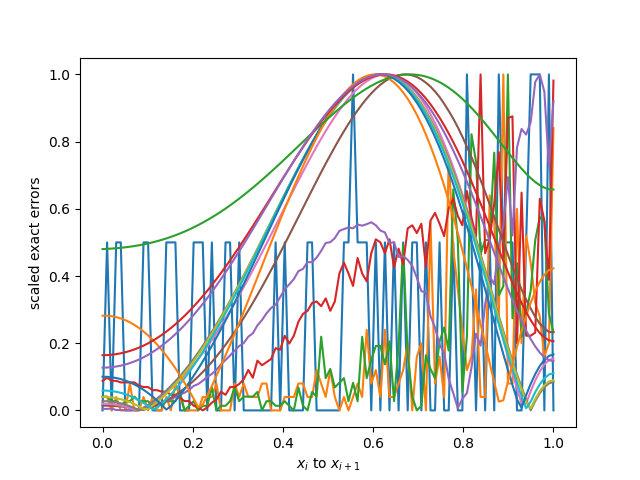
\includegraphics[width=0.7\linewidth]{./figures/rk6_with_hb6_hb8_sampling_p2_scaled_errors}
\caption{Scaled errors over all steps for RK6 with HB6 vs HB8 with error sampling on problem 2 at an absolute tolerance of $10^{-6}$ mapped onto $[0, 1]$.}
\label{fig:rk6_with_hb6_hb8_sampling_p2_scaled_errors}
\end{figure}

\paragraph{Problem 3} Figures $\ref{fig:rk6_with_hb6_hb8_sampling_p3_global_error}$ and $\ref{fig:rk6_with_hb6_hb8_sampling_p3_scaled_errors}$ shows the global error and the shape of the error on each step of using rk6 with hb6 vs hb8 with sampling on Problem 3 at an absolute tolerance of $10^{-6}$. From Figure $\ref{fig:rk6_with_hb6_hb8_sampling_p3_scaled_errors}$, we can see that there is no consistent location where we can sample the error to get the maximum error.

\begin{figure}[H]
\centering
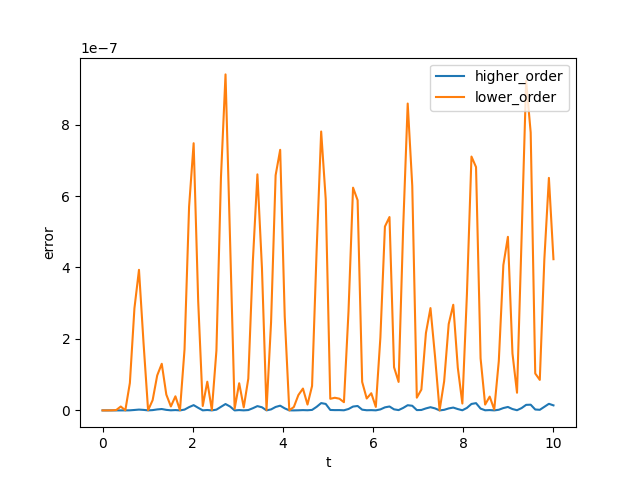
\includegraphics[width=0.7\linewidth]{./figures/rk6_with_hb6_hb8_sampling_p3_global_error}
\caption{Global Error for RK6 with HB6 vs HB8 with error sampling on problem 3 at an absolute tolerance of $10^{-6}$.}
\label{fig:rk6_with_hb6_hb8_sampling_p3_global_error}
\end{figure}

\begin{figure}[H]
\centering
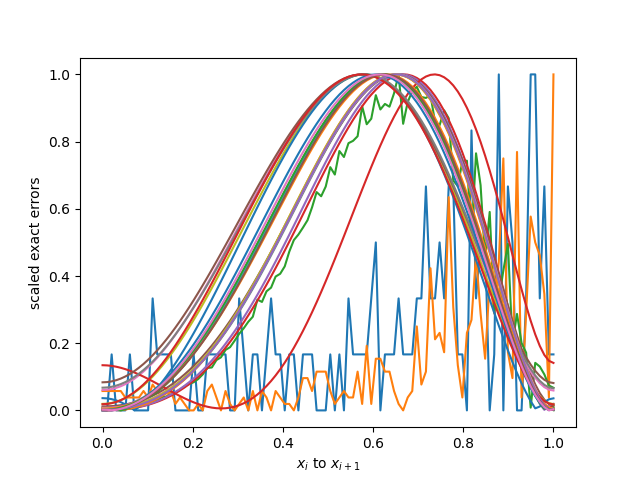
\includegraphics[width=0.7\linewidth]{./figures/rk6_with_hb6_hb8_sampling_p3_scaled_errors}
\caption{Scaled errors over all steps for RK6 with HB6 vs HB8 with error sampling on problem 3 at an absolute tolerance of $10^{-6}$ mapped onto $[0, 1]$.}
\label{fig:rk6_with_hb6_hb8_sampling_p3_scaled_errors}
\end{figure}

\begin{table}[h]
\caption {Number of steps taken by RK6 using error control with HB6 vs HB8 by sampling the error.} \label{tab:rk6_with_hb6_hb8_sampling_nsteps}
\begin{center}
\begin{tabular}{ c c c } 
Problem & successful steps & total steps \\ 
1       & 17                         & 17 \\ 
2       & 15                         & 21 \\
3       & 27                         & 34 \\
\end{tabular}
\end{center}
\end{table}

\subsection{Problems with error sampling.}
The shape of the error across each step is very inconsistent (See the Scaled errors plots in the previous section).One idea would be to find the max error by sampling at even more points. However, a lot of samplings would be required to reach a consistent error estimate scheme. In the next section, we present a way to sample the error using a continuous L2 norm. This essentially measures the distance between the two interpolants. By designing a continuous L2-norm scheme that maintain ratio of the error estimate from an L2 norm between two interpolants and the actual error between the interpolant and the actual solution, we guarantee that controlling the L2 norm controls the global error.

\subsection{continuous L2 norm}
The error estimate is calculated with a continuous L2 norm as follows.
\begin{equation}
estimated\_error_i = \sqrt{ \int_{x_i}^{x_{i+1}} (\frac{h(x) - l(x)}{1 + |l(x)|})^2 \,dx }
\end{equation}
where h(x) is the higher order interpolant and l(x) is the lower order interpolant. This formula gives the error for one step and we compare it with the user provided atol for error control. 

========================
We ignored rtol as we had to factorise tol from the denominator so that we can use tol and $tol/10$ for comparisons. Essentially we assume $atol == rtol$
===================

We note that the solver performs error control through the continuous L2 norm but we want to control the actual error between the exact solution and the interpolant that was returned. To that effect, we define the following ratio: $\frac{estimated\_error_i}{exact\_error_i}$. Ideally, we want this ratio to be 1 for the scheme that we designed as a ratio of 1 entails that controlling the L2-norm would control the error between the interpolant and the exact solution.

We note that we consider the exact error is calculated with
\begin{equation}
exact\_error_i = \sqrt{ \int_{x_i}^{x_{i+1}} (\frac{sol(x) - l(x)}{1 + |l(x)|})^2 \,dx }
\end{equation}
where $sol(x)$ is the solution at point, x so that we can plot $\frac{estimated\_error_i}{exact\_error_i}$. 

To perform the integration, we use a Gauss rule. Through experimentation, we have seen that a 3-point Gauss rule was enough to produce efficient solution. A 2-point rule increased was being affected by the integration error whereas 4- and 5-points rules were not improving the number of steps taken by much showing that the integration error was no longer a limiting factor as from the 3-point rule. We note that we want to use as the smallest Gauss rule we can get away with to improve efficiency.

\subsubsection{rk4 with hb4 vs hb6 with continuous L2 norm}
Because we do not differentiate and that hb4 has order 4, we can use with rk4 with HB4 for error control. Thus HB4 and HB6 should not suffer from much interpolation error and we can use rk4 with the hb4 and hb6 using the error scheme


\paragraph{Problem 1} Figures $\ref{fig:rk4_with_hb4_hb6_L2norm_p1_global_error}$ and $\ref{fig:rk4_with_hb4_hb6_L2norm_p1_error_ratio}$ shows the global error and the ratio $\frac{estimated\_error_i}{exact\_error_i}$ on each step of using rk4 with hb4 vs hb6 with continuous L2 norm on Problem 1 at an absolute tolerance of $10^{-6}$. From Figure $\ref{fig:rk4_with_hb4_hb6_L2norm_p1_error_ratio}$, we can see that the ratio is relatively close to 1 and we can see in Figure  $\ref{fig:rk4_with_hb4_hb6_L2norm_p1_global_error}$ that the exact error is within the tolerance even when the continuous L2 norm between the two interpolant was used to control the error.

\begin{figure}[H]
\centering
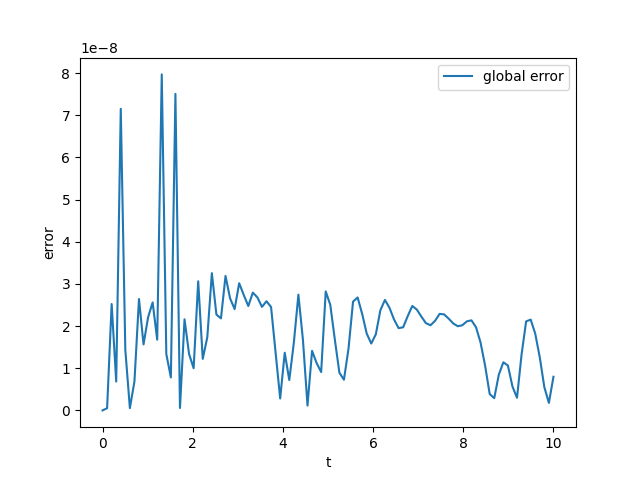
\includegraphics[width=0.7\linewidth]{./figures/rk4_with_hb4_hb6_L2norm_p1_global_error}
\caption{Global Error for RK4 with HB4 vs HB6 with continuous L2 norm on problem 1 at an absolute tolerance of $10^{-6}$.}
\label{fig:rk4_with_hb4_hb6_L2norm_p1_global_error}
\end{figure}

\begin{figure}[H]
\centering
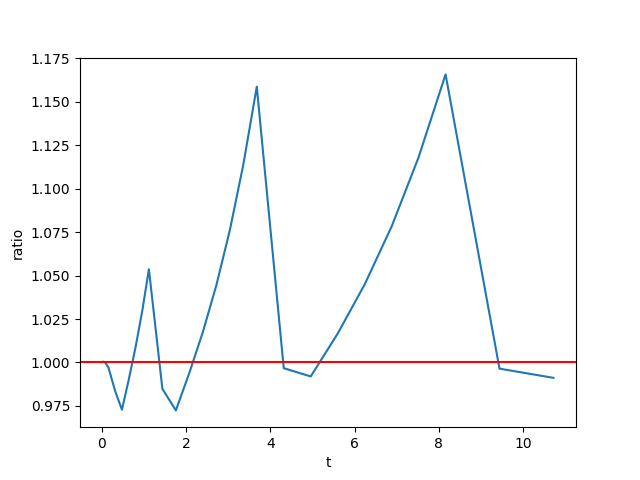
\includegraphics[width=0.7\linewidth]{./figures/rk4_with_hb4_hb6_L2norm_p1_error_ratio}
\caption{Ratio $\frac{estimated\_error_i}{exact\_error_i}$ at the end of each successful step for RK4 with HB4 vs HB6 with continuous L2 norm on problem 1 at an absolute tolerance of $10^{-6}$.}
\label{fig:rk4_with_hb4_hb6_L2norm_p1_error_ratio}
\end{figure}

\paragraph{Problem 2} Figures $\ref{fig:rk4_with_hb4_hb6_L2norm_p2_global_error}$ and $\ref{fig:rk4_with_hb4_hb6_L2norm_p2_error_ratio}$ shows the global error and the ratio $\frac{estimated\_error_i}{exact\_error_i}$ on each step of using rk4 with hb4 vs hb6 with continuous L2 norm on Problem 2 at an absolute tolerance of $10^{-6}$. From Figure $\ref{fig:rk4_with_hb4_hb6_L2norm_p2_error_ratio}$, we can see that the ratio is not relatively close to 1 and we can see in Figure $\ref{fig:rk4_with_hb4_hb6_L2norm_p2_global_error}$ that the exact error is not within the tolerance.

\begin{figure}[H]
\centering
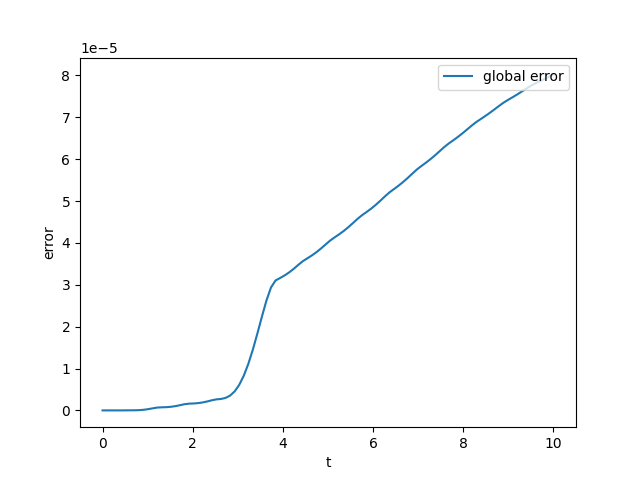
\includegraphics[width=0.7\linewidth]{./figures/rk4_with_hb4_hb6_L2norm_p2_global_error}
\caption{Global Error for RK4 with HB4 vs HB6 with continuous L2 norm on problem 2 at an absolute tolerance of $10^{-6}$.}
\label{fig:rk4_with_hb4_hb6_L2norm_p2_global_error}
\end{figure}

\begin{figure}[H]
\centering
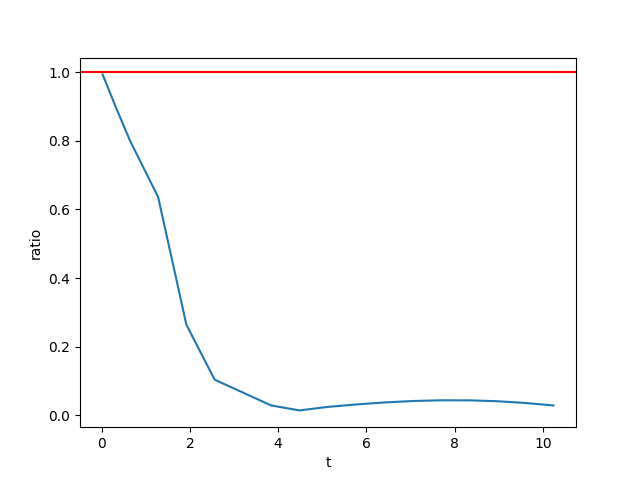
\includegraphics[width=0.7\linewidth]{./figures/rk4_with_hb4_hb6_L2norm_p2_error_ratio}
\caption{Ratio $\frac{estimated\_error_i}{exact\_error_i}$ at the end of each successful step for RK4 with HB4 vs HB6 with continuous L2 norm on problem 2 at an absolute tolerance of $10^{-6}$.}
\label{fig:rk4_with_hb4_hb6_L2norm_p2_error_ratio}
\end{figure}

\paragraph{Problem 3} Figures $\ref{fig:rk4_with_hb4_hb6_L2norm_p3_global_error}$ and $\ref{fig:rk4_with_hb4_hb6_L2norm_p3_error_ratio}$ shows the global error and the ratio $\frac{estimated\_error_i}{exact\_error_i}$ on each step of using rk4 with hb4 vs hb6 with continuous L2 norm on Problem 3 at an absolute tolerance of $10^{-6}$. From Figure $\ref{fig:rk4_with_hb4_hb6_L2norm_p3_error_ratio}$, we can see that the ratio is relatively close to 1 and we can see in Figure  $\ref{fig:rk4_with_hb4_hb6_L2norm_p3_global_error}$ that the exact error is within the tolerance even when the continuous L2 norm between the two interpolant was used to control the error.

\begin{figure}[H]
\centering
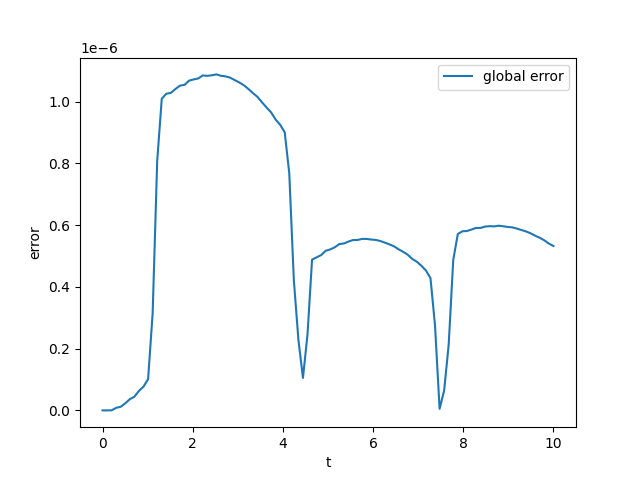
\includegraphics[width=0.7\linewidth]{./figures/rk4_with_hb4_hb6_L2norm_p3_global_error}
\caption{Global Error for RK4 with HB4 vs HB6 with continuous L2 norm on problem 3 at an absolute tolerance of $10^{-6}$.}
\label{fig:rk4_with_hb4_hb6_L2norm_p3_global_error}
\end{figure}

\begin{figure}[H]
\centering
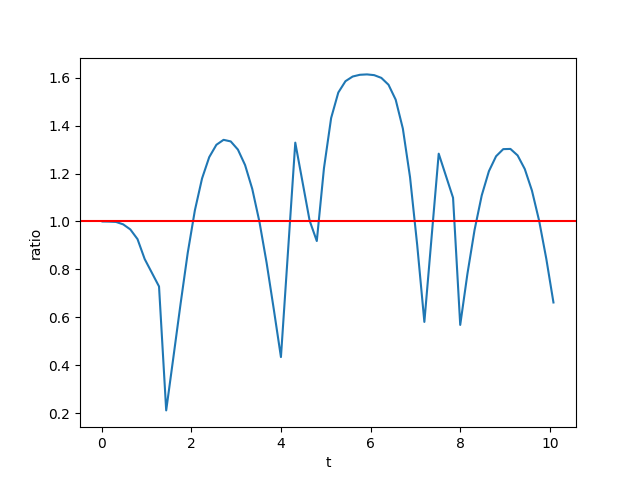
\includegraphics[width=0.7\linewidth]{./figures/rk4_with_hb4_hb6_L2norm_p3_error_ratio}
\caption{Ratio $\frac{estimated\_error_i}{exact\_error_i}$ at the end of each successful step for RK4 with HB4 vs HB6 with continuous L2 norm on problem 3 at an absolute tolerance of $10^{-6}$.}
\label{fig:rk4_with_hb4_hb6_L2norm_p3_error_ratio}
\end{figure}

\begin{table}[h]
\caption {Number of steps taken by RK4 using error control with HB4 vs HB6 by using a continuous L2 norm.} \label{tab:rk4_with_hb4_hb6_L2norm_nsteps}
\begin{center}
\begin{tabular}{ c c c } 
Problem & successful steps & total steps \\ 
1       & 27                         & 29 \\ 
2       & 20                         & 21 \\
3       & 61                         & 68 \\
\end{tabular}
\end{center}
\end{table}

\subsubsection{rk4 with hb6 vs hb8 with continuous L2 norm}
rk4 can also be use with hb6  and hb8 and not suffer from much interpolation error.



\paragraph{Problem 1} Figures $\ref{fig:rk4_with_hb6_hb8_L2norm_p1_global_error}$ and $\ref{fig:rk4_with_hb6_hb8_L2norm_p1_error_ratio}$ shows the global error and the ratio $\frac{estimated\_error_i}{exact\_error_i}$ on each step of using rk4 with hb6 vs hb8 with continuous L2 norm on Problem 1 at an absolute tolerance of $10^{-6}$. From Figure $\ref{fig:rk4_with_hb6_hb8_L2norm_p1_error_ratio}$, we can see that the ratio is relatively close to 1 and we can see in Figure  $\ref{fig:rk4_with_hb6_hb8_L2norm_p1_global_error}$ that the exact error is within the tolerance even when the continuous L2 norm between the two interpolant was used to control the error.

\begin{figure}[H]
\centering
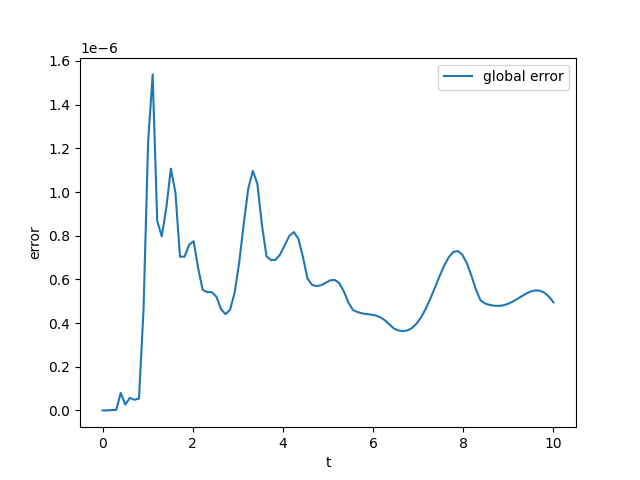
\includegraphics[width=0.7\linewidth]{./figures/rk4_with_hb6_hb8_L2norm_p1_global_error}
\caption{Global Error for RK4 with HB6 vs HB8 with continuous L2 norm on problem 1 at an absolute tolerance of $10^{-6}$.}
\label{fig:rk4_with_hb6_hb8_L2norm_p1_global_error}
\end{figure}

\begin{figure}[H]
\centering
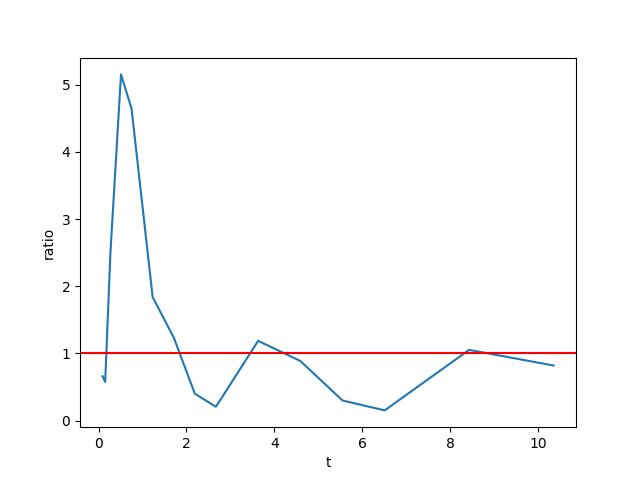
\includegraphics[width=0.7\linewidth]{./figures/rk4_with_hb6_hb8_L2norm_p1_error_ratio}
\caption{Ratio $\frac{estimated\_error_i}{exact\_error_i}$ at the end of each successful step for RK4 with HB6 vs HB8 with continuous L2 norm on problem 1 at an absolute tolerance of $10^{-6}$.}
\label{fig:rk4_with_hb6_hb8_L2norm_p1_error_ratio}
\end{figure}

\paragraph{Problem 2} Figures $\ref{fig:rk4_with_hb6_hb8_L2norm_p2_global_error}$ and $\ref{fig:rk4_with_hb6_hb8_L2norm_p2_error_ratio}$ shows the global error and the ratio $\frac{estimated\_error_i}{exact\_error_i}$ on each step of using rk4 with hb6 vs hb8 with continuous L2 norm on Problem 2 at an absolute tolerance of $10^{-6}$. From Figure $\ref{fig:rk4_with_hb6_hb8_L2norm_p2_error_ratio}$, we can see that the ratio is not relatively close to 1 and we can see in Figure $\ref{fig:rk4_with_hb6_hb8_L2norm_p2_global_error}$ that the exact error is not within the tolerance.

\begin{figure}[H]
\centering
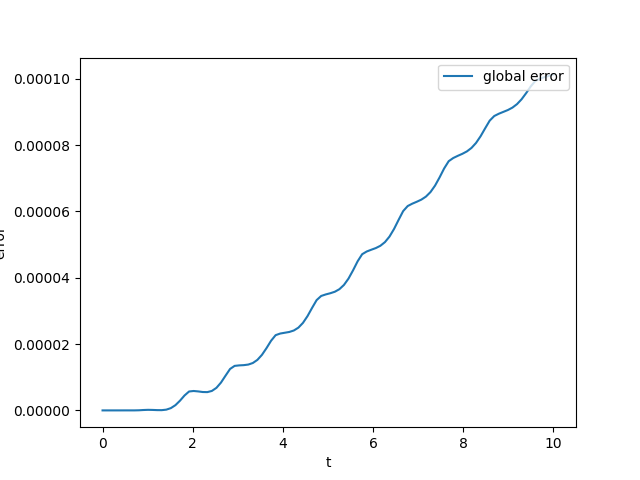
\includegraphics[width=0.7\linewidth]{./figures/rk4_with_hb6_hb8_L2norm_p2_global_error}
\caption{Global Error for RK4 with HB6 vs HB8 with continuous L2 norm on problem 2 at an absolute tolerance of $10^{-6}$.}
\label{fig:rk4_with_hb6_hb8_L2norm_p2_global_error}
\end{figure}

\begin{figure}[H]
\centering
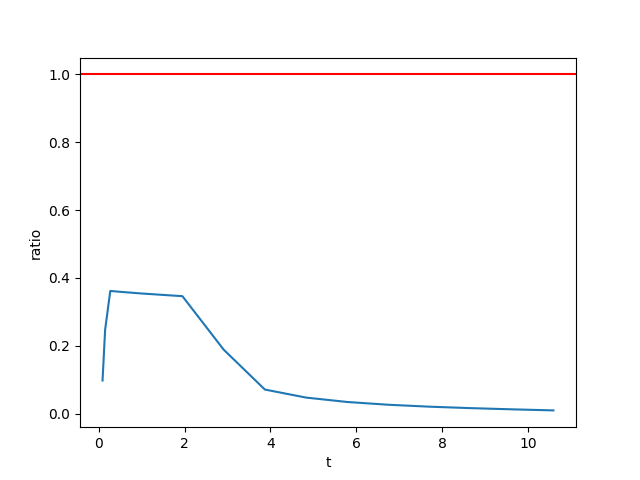
\includegraphics[width=0.7\linewidth]{./figures/rk4_with_hb6_hb8_L2norm_p2_error_ratio}
\caption{Ratio $\frac{estimated\_error_i}{exact\_error_i}$ at the end of each successful step for RK4 with HB6 vs HB8 with continuous L2 norm on problem 2 at an absolute tolerance of $10^{-6}$.}
\label{fig:rk4_with_hb6_hb8_L2norm_p2_error_ratio}
\end{figure}

\paragraph{Problem 3} Figures $\ref{fig:rk4_with_hb6_hb8_L2norm_p3_global_error}$ and $\ref{fig:rk4_with_hb6_hb8_L2norm_p3_error_ratio}$ shows the global error and the ratio $\frac{estimated\_error_i}{exact\_error_i}$ on each step of using rk4 with hb6 vs hb8 with continuous L2 norm on Problem 3 at an absolute tolerance of $10^{-6}$. From Figure $\ref{fig:rk4_with_hb6_hb8_L2norm_p3_error_ratio}$, we can see that the ratio is not relatively close to 1 and we can see in Figure $\ref{fig:rk4_with_hb6_hb8_L2norm_p3_global_error}$ that the exact error is not within the tolerance.


\begin{figure}[H]
\centering
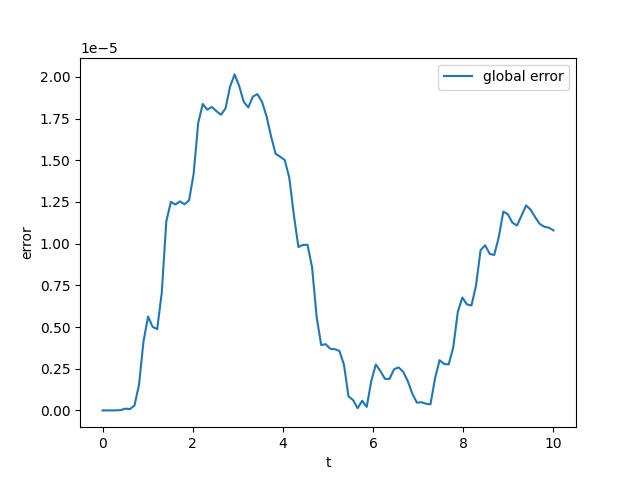
\includegraphics[width=0.7\linewidth]{./figures/rk4_with_hb6_hb8_L2norm_p3_global_error}
\caption{Global Error for RK4 with HB6 vs HB8 with continuous L2 norm on problem 3 at an absolute tolerance of $10^{-6}$.}
\label{fig:rk4_with_hb6_hb8_L2norm_p3_global_error}
\end{figure}

\begin{figure}[H]
\centering
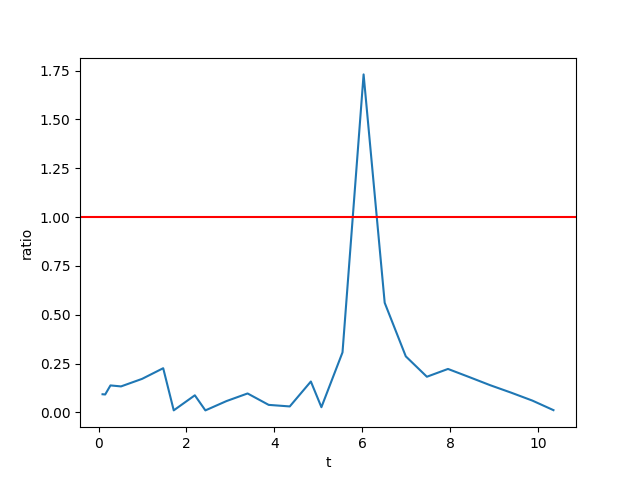
\includegraphics[width=0.7\linewidth]{./figures/rk4_with_hb6_hb8_L2norm_p3_error_ratio}
\caption{Ratio $\frac{estimated\_error_i}{exact\_error_i}$ at the end of each successful step for RK4 with HB6 vs HB8 with continuous L2 norm on problem 3 at an absolute tolerance of $10^{-6}$.}
\label{fig:rk4_with_hb6_hb8_L2norm_p3_error_ratio}
\end{figure}

\begin{table}[h]
\caption {Number of steps taken by RK4 using error control with HB6 vs HB8 by using a continuous L2 norm.} \label{tab:rk4_with_hb6_hb8_L2norm_nsteps}
\begin{center}
\begin{tabular}{ c c c } 
Problem & successful steps & total steps \\ 
1       & 15                         & 16 \\ 
2       & 15                         & 15 \\
3       & 26                         & 29 \\
\end{tabular}
\end{center}
\end{table}


\subsubsection{rk6 with hb6 vs hb8 with continuous L2 norm}
Because we do not differentiate and that hb6 has order 6, we can use with rk6 with HB6 for error control. Thus HB6 and HB8 should not suffer from much interpolation error and we can use rk6 with the hb4 and hb6 using the error scheme.

\paragraph{Problem 1} Figures $\ref{fig:rk6_with_hb6_hb8_L2norm_p1_global_error}$ and $\ref{fig:rk6_with_hb6_hb8_L2norm_p1_error_ratio}$ shows the global error and the ratio $\frac{estimated\_error_i}{exact\_error_i}$ on each step of using rk6 with hb6 vs hb8 with continuous L2 norm on Problem 1 at an absolute tolerance of $10^{-6}$. From Figure $\ref{fig:rk6_with_hb6_hb8_L2norm_p1_error_ratio}$, we can see that the ratio is relatively close to 1 and we can see in Figure $\ref{fig:rk6_with_hb6_hb8_L2norm_p1_global_error}$ that the exact error is within the tolerance even when the continuous L2 norm between the two interpolant was used to control the error.

\begin{figure}[H]
\centering
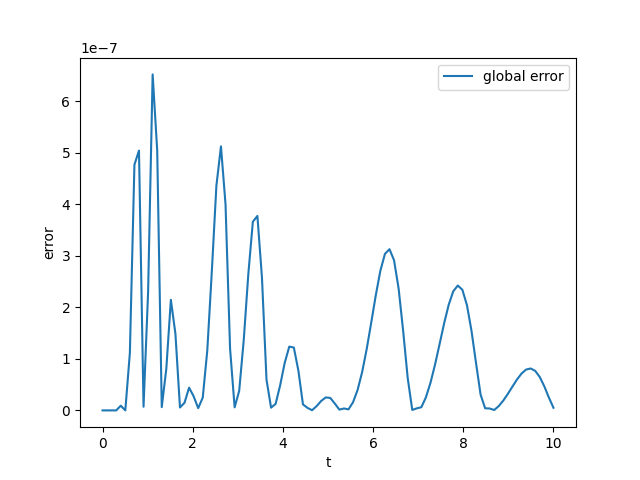
\includegraphics[width=0.7\linewidth]{./figures/rk6_with_hb6_hb8_L2norm_p1_global_error}
\caption{Global Error for RK6 with HB6 vs HB8 with continuous L2 norm on problem 1 at an absolute tolerance of $10^{-6}$.}
\label{fig:rk6_with_hb6_hb8_L2norm_p1_global_error}
\end{figure}

\begin{figure}[H]
\centering
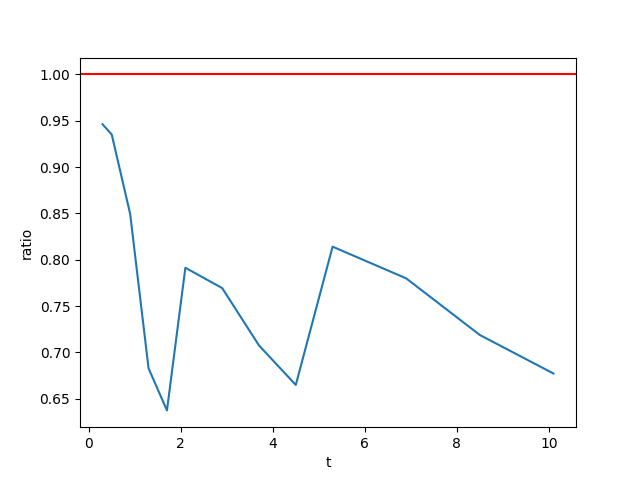
\includegraphics[width=0.7\linewidth]{./figures/rk6_with_hb6_hb8_L2norm_p1_error_ratio}
\caption{Ratio $\frac{estimated\_error_i}{exact\_error_i}$ at the end of each successful step for RK6 with HB6 vs HB8 with continuous L2 norm on problem 1 at an absolute tolerance of $10^{-6}$.}
\label{fig:rk6_with_hb6_hb8_L2norm_p1_error_ratio}
\end{figure}

\paragraph{Problem 2} Figures $\ref{fig:rk6_with_hb6_hb8_L2norm_p2_global_error}$ and $\ref{fig:rk6_with_hb6_hb8_L2norm_p2_error_ratio}$ shows the global error and the ratio $\frac{estimated\_error_i}{exact\_error_i}$ on each step of using rk6 with hb6 vs hb8 with continuous L2 norm on Problem 2 at an absolute tolerance of $10^{-6}$. From Figure $\ref{fig:rk6_with_hb6_hb8_L2norm_p2_error_ratio}$, we can see that the ratio is relatively close to 1 and we can see in Figure $\ref{fig:rk6_with_hb6_hb8_L2norm_p2_global_error}$ that the exact error is within the tolerance even when the continuous L2 norm between the two interpolant was used to control the error.

\begin{figure}[H]
\centering
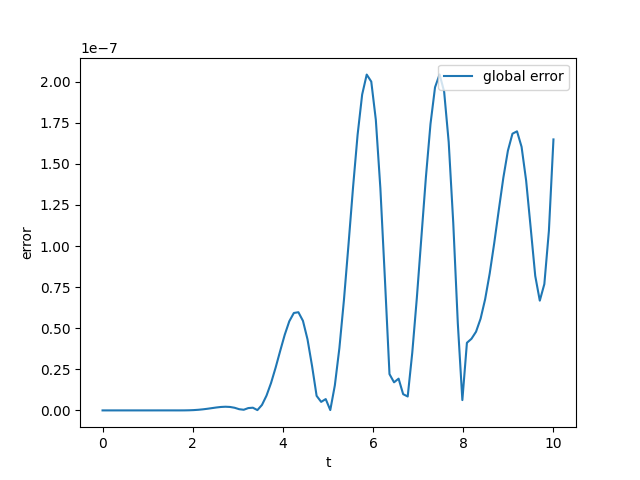
\includegraphics[width=0.7\linewidth]{./figures/rk6_with_hb6_hb8_L2norm_p2_global_error}
\caption{Global Error for RK6 with HB6 vs HB8 with continuous L2 norm on problem 2 at an absolute tolerance of $10^{-6}$.}
\label{fig:rk6_with_hb6_hb8_L2norm_p2_global_error}
\end{figure}

\begin{figure}[H]
\centering
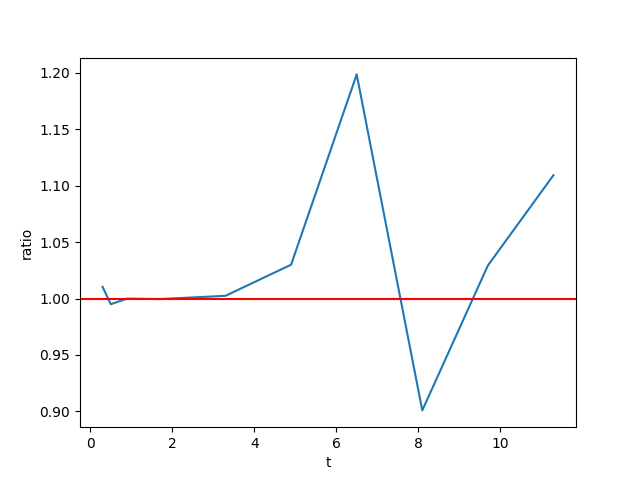
\includegraphics[width=0.7\linewidth]{./figures/rk6_with_hb6_hb8_L2norm_p2_error_ratio}
\caption{Ratio $\frac{estimated\_error_i}{exact\_error_i}$ at the end of each successful step for RK6 with HB6 vs HB8 with continuous L2 norm on problem 2 at an absolute tolerance of $10^{-6}$.}
\label{fig:rk6_with_hb6_hb8_L2norm_p2_error_ratio}
\end{figure}

\paragraph{Problem 3} Figures $\ref{fig:rk6_with_hb6_hb8_L2norm_p3_global_error}$ and $\ref{fig:rk6_with_hb6_hb8_L2norm_p3_error_ratio}$ shows the global error and the ratio $\frac{estimated\_error_i}{exact\_error_i}$ on each step of using rk6 with hb6 vs hb8 with continuous L2 norm on Problem 3 at an absolute tolerance of $10^{-6}$. From Figure $\ref{fig:rk6_with_hb6_hb8_L2norm_p3_error_ratio}$, we can see that the ratio is relatively close to 1 and we can see in Figure $\ref{fig:rk6_with_hb6_hb8_L2norm_p3_global_error}$ that the exact error is within the tolerance even when the continuous L2 norm between the two interpolant was used to control the error.


\begin{figure}[H]
\centering
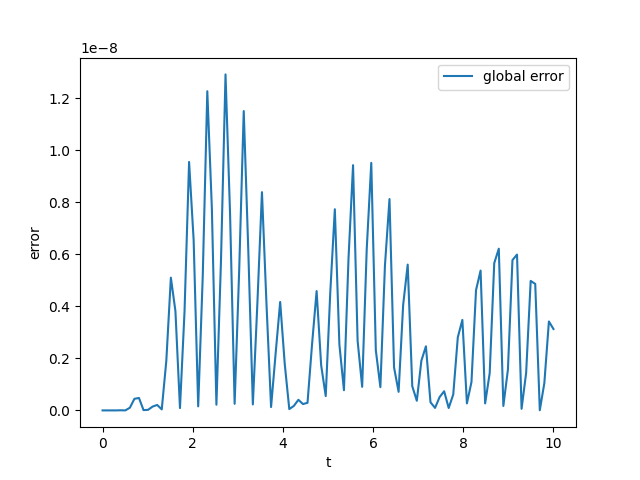
\includegraphics[width=0.7\linewidth]{./figures/rk6_with_hb6_hb8_L2norm_p3_global_error}
\caption{Global Error for RK6 with HB6 vs HB8 with continuous L2 norm on problem 3 at an absolute tolerance of $10^{-6}$.}
\label{fig:rk6_with_hb6_hb8_L2norm_p3_global_error}
\end{figure}

\begin{figure}[H]
\centering
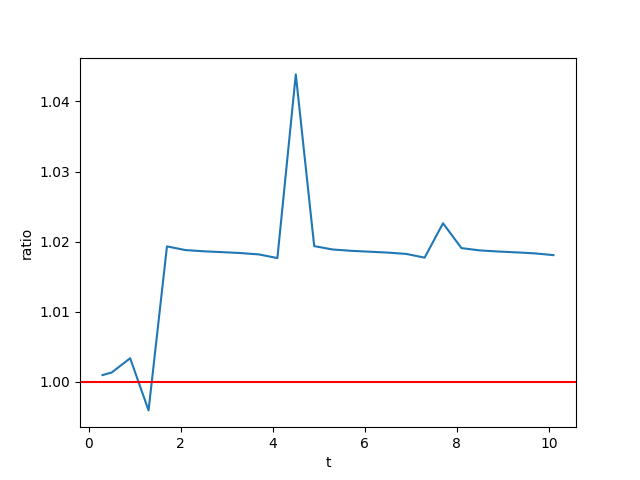
\includegraphics[width=0.7\linewidth]{./figures/rk6_with_hb6_hb8_L2norm_p3_error_ratio}
\caption{Ratio $\frac{estimated\_error_i}{exact\_error_i}$ at the end of each successful step for RK6 with HB6 vs HB8 with continuous L2 norm on problem 3 at an absolute tolerance of $10^{-6}$.}
\label{fig:rk6_with_hb6_hb8_L2norm_p3_error_ratio}
\end{figure}

\begin{table}[h]
\caption {Number of steps taken by RK6 using error control with HB6 vs HB8 by using a continuous L2 norm.} \label{tab:rk6_with_hb6_hb8_L2norm_nsteps}
\begin{center}
\begin{tabular}{ c c c } 
Problem & successful steps & total steps \\ 
1       & 13                         & 15 \\ 
2       & 10                         & 10 \\
3       & 26                         & 36 \\
\end{tabular}
\end{center}
\end{table}

========================================================================================
Hello Prof.
The figures and the number of steps for RK6 using error control with HB6 vs HB8 by using a continuous L2 norm are extremely good. The solution is both very accurate and very efficient compared to everything we have so far.... What is even more impressive is that we can solve very efficiently at 1e-12, we are talking 2 to 3 times more efficient than rk6 with HB8 defect control.

\begin{table}[h]
\caption {Number of steps taken by RK6 using error control with HB6 vs HB8 by using a continuous L2 norm at a tolerance of $10^{-12}$.} \label{tab:rk6_with_hb6_hb8_L2norm_compared}
\begin{center}
\begin{tabular}{ c c c } 
Problem & successful steps & total steps \\ 
1       & 109vs261            & 158vs290 \\ 
2       & 50vs134             & 53vs196 \\
3       & 189vs297            & 236vs466 \\
\end{tabular}
\end{center}
\end{table}

Table $\ref{tab:rk6_with_hb6_hb8_L2norm_compared}$ shows the comparison between rk6 with hb6 vs hb8 with L2 norm and rk6 with hb8 defect control. We note that the solution for rk6 with hb6 vs hb8 with L2 norm keeps the global error within $10^{-12}$.
========================================================================================================
\subsection{conclusion}
The continuous L2 norm works expect from Problem 2 where the ratio is often off. We note that Problem 2 has an exponentially growing solution. A better error estimate that takes this into account may help the situation.

rk6 with hb6 vs hb8 using a continuous L2 norm is very efficient and accurate and should be explored further.